% !TeX root = RJwrapper.tex
\title{\pkg{jsr223}: A Java Platform Integration for R with Programming Languages Groovy, JavaScript, JRuby, Jython, and Kotlin}
\author{by Floid R. Gilbert and David B. Dahl}

\maketitle

\abstract{
The R package \CRANpkg{jsr223} is a high-level integration for the Java platform that makes Java objects easy to use from within R; provides a unified interface to integrate R with several programming languages; and features extensive data exchange between R and Java. In all, \pkg{jsr223} significantly extends the computing capabilities of the R software environment.
}

%///put new example in repo. update repo info. remember subfolder is engines. not sure if that is nec. with maven these days.
%///synchronize user manual with this document.
%///review bib. need to add DL4J. treebank is broken. need better citation.
%///update kotlin manual to use maven
%//////make sure class path doesn't get to github.
%///DOI

\hypertarget{introduction}{}
\section{Introduction}

About the same time Ross Ihaka and Robert Gentleman began developing R at the University of Auckland in the early 1990s, James Gosling and the so-called Green Project Team was working on a new programming language at Sun Microsystems in California. The Green Team did not set out to make a new language; rather, they were trying to move platform-independent, distributed computing into the consumer electronics marketplace. As Gosling explained, ``All along, the language was a tool, not the end'' \citep{javainsidestory}. Unexpectedly, the programming language outlived the Green Project and sparked one of the most successful development platforms in computing history: Java. According to the \href{https://www.tiobe.com/tiobe-index/}{TIOBE index}, Java has been the most popular programming language, on average, over the last sixteen years. Java's success can be attributed to several factors. Perhaps the most important factor is platform-independence: the same Java program can run on several operating systems and hardware devices. Another important factor is that memory management is handled automatically for the programmer. Consequently, Java programs are easier to write and have fewer memory-related bugs than programs written in C/C++. These and other factors accelerated Java's adoption in enterprise systems which, in turn, established a thriving developer community that has created production-quality frameworks, libraries, and programming languages for the Java platform. Many successful Java solutions are relevant to data science today such as \href{http://hadoop.apache.org/}{Hadoop}, \href{https://hive.apache.org/}{Hive}, \href{https://spark.apache.org/}{Spark}, \href{http://cassandra.apache.org/}{Cassandra}, \href{https://hbase.apache.org/}{HBase}, \href{https://mahout.apache.org/}{Mahout}, \href{https://deeplearning4j.org/}{Deeplearning4j}, \href{https://stanfordnlp.github.io/CoreNLP/}{Stanford CoreNLP}, and others.

In 2003, Simon Urbanek released \CRANpkg{rJava} \citeyearpar{rjava}, an integration package designed to avail R of the burgeoning development surrounding Java. The package has been very successful to this end. Today, it is one of the top-ranked solutions for R as measured by monthly downloads.\footnote{\pkg{rJava} ranks in the $99^{\text{th}}$ percentile for R package downloads according to \url{http://rdocumentation.org}.} \pkg{rJava} is described by Urbanek as a low-level R to Java interface analogous to \code{.C} and \code{.Call}, the built-in R functions for calling compiled C code. Like R's integration for C, \pkg{rJava} loads compiled code into an R process's memory space where it can be accessed via various R functions. Urbanek achieves this feat using the Java Native Interface (JNI), a standard framework that enables native (i.e. platform-dependent) code to access and use compiled Java code. The \pkg{rJava} API requires users to specify classes and data types in JNI syntax. One advantage to this approach is that it gives users granular, direct access to Java classes. However, as with any low-level interface, the learning curve is relatively high and implementation requires verbose coding. A second advantage to using JNI is that it avoids the difficult task of dynamically interpreting or compiling source code. Of course, this is also a disadvantage: it limits \pkg{rJava} to using compiled code as opposed to embedding source code directly within R script.

Our \CRANpkg{jsr223} package builds on \pkg{rJava} to provide a high-level interface to the Java platform. We accomplish this by embedding other programming languages in R that use Java objects in natural syntax. As we show in the \hyperlink{rjava-software-review}{``\pkg{rJava} software review''}, this approach is generally simpler and more intuitive than \pkg{rJava}'s low-level JNI interface. To date, \pkg{jsr223} supports embedding five programming languages: Groovy, JavaScript, JRuby, Jython, and Kotlin. (JRuby and Jython are Java platform implementations of the Ruby and Python languages, respectively.) See Table \ref{tab:programming-languages} for a brief description of each language.

The \pkg{jsr223} multi-language integration is made possible by the Java Scripting API \citep{jsa}, an implementation of the specification “JSR-223: Scripting for the Java Platform” \citep{jsr223spec}. The JSR-223 specification includes two crucial elements: an interface for Java applications to execute code written in scripting languages, and a guide for scripting languages to create Java objects in their own syntax. Hence, JSR-223 is the basis for our package. However, no knowledge of JSR-223 or the Java Scripting API is necessary to use \pkg{jsr223}. Figures \ref{fig:scheme-rjava} and \ref{fig:scheme-jsr223} show how \pkg{rJava} and \pkg{jsr223} facilitate access to the Java platform. Where \pkg{rJava} uses JNI, \pkg{jsr223} uses the Java Scripting API and embeddable programming languages.

\begin{figure}[h]
\centering
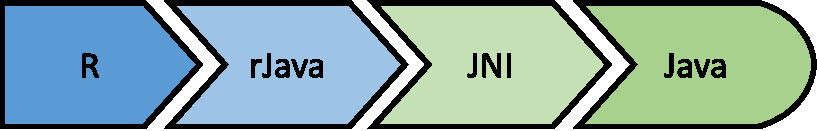
\includegraphics[width=0.40\linewidth]{scheme-rjava}
\caption{The \pkg{rJava} package facilitates low-level access to the Java platform through the Java Native Interface (JNI). Some knowledge of JNI is required.}
\label{fig:scheme-rjava}
\end{figure}

\begin{figure}[h]
\centering
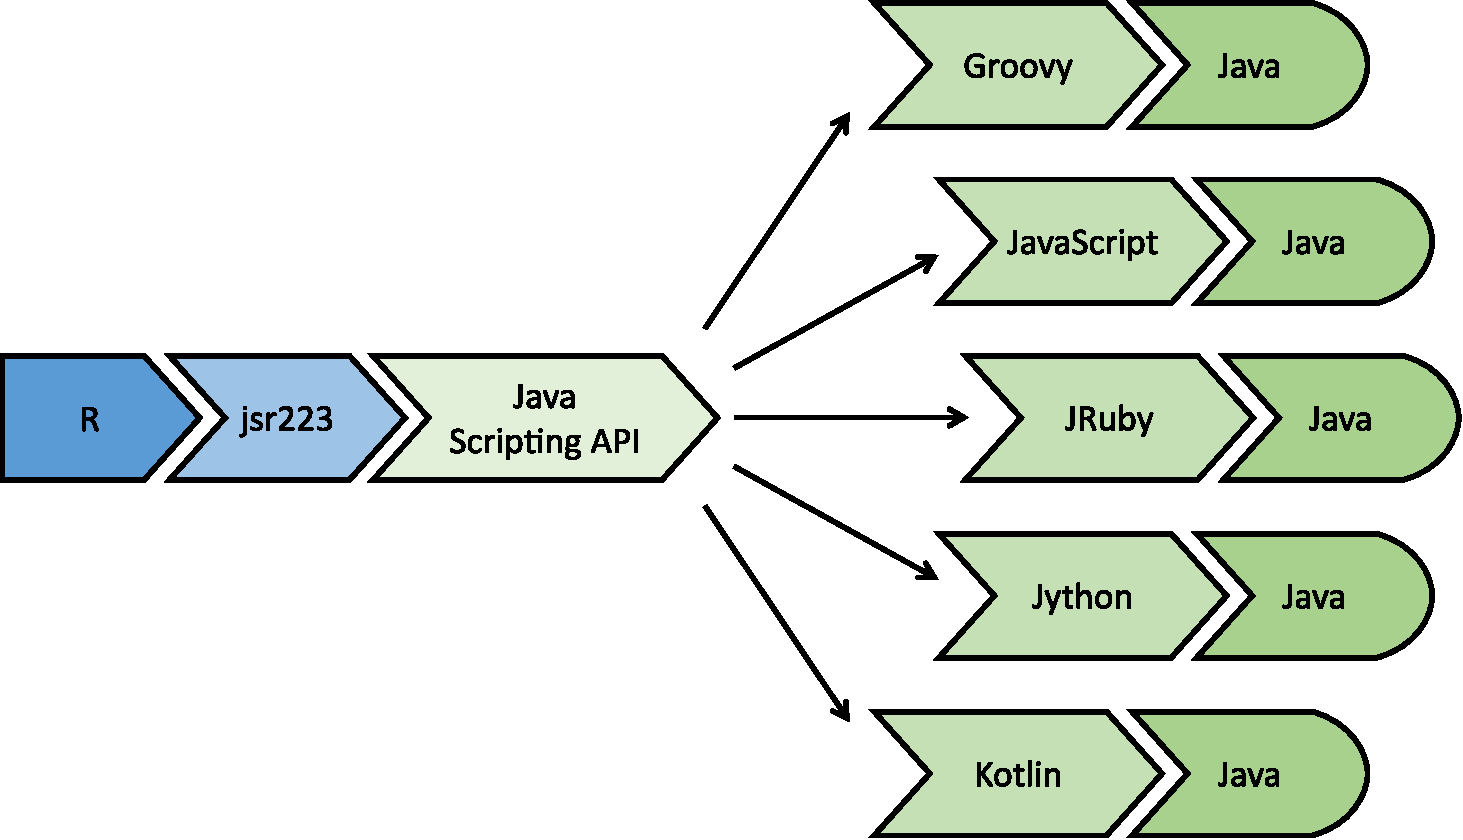
\includegraphics[width=.72\linewidth]{scheme-jsr223}
\caption{The \pkg{jsr223} package provides high-level access to the Java platform through five programming languages. \pkg{jsr223} presents a unified interface to these languages by merit of the Java Scripting API. Knowledge of the Java Scripting API is not required to use \pkg{jsr223}.}
\label{fig:scheme-jsr223}
\end{figure}

The primary goal of \pkg{jsr223} is to enable R developers to leverage existing Java solutions with relative ease. We demonstrate two typical use cases in this document with subjects that are of particular interest to many data scientists: a natural language processor, and a neural network classifier. In addition to Java solutions, R developers can use projects developed in any of the five \pkg{jsr223}-supported programming languages. In essence, \pkg{jsr223} opens R to a broader ecosystem.

For Java developers, \pkg{jsr223} facilitates writing high-performance, cross-platform R extensions using their preferred platform. \pkg{jsr223} also allows organizations that run enterprise Java applications to more readily develop dashboards and other business intelligence tools. Instead of writing R code to query raw data from a database, \pkg{jsr223} enables R packages to consume data directly from their application's Java object model where the data has been coalesced according to business rules. Java developers will also be interested to know that the \pkg{jsr223}-supported programming languages can implement interfaces and extend classes, just like the Java programming language. and compiling. See ``Extending existing Java solutions'' in the \textit{\pkg{jsr223} User Manual} for an in-depth code example that demonstrates extending Java classes and several other features.

///Insert some concluding statement for the introduction.

\begin{table}[t]
\centering
\caption{The five programming languages supported by \pkg{jsr223}. See the \textit{\pkg{jsr223} User Manual} for code examples and language details.}
\begin{tabular}{p{2cm} p{11cm}}
\toprule
\textbf{Language} & \textbf{Description} \\ \midrule
\noalign{\vspace{1ex}}
\href{http://groovy-lang.org}{Groovy} &  Groovy is a scripting language that follows Java syntax very closely. Hence, \pkg{jsr223} enables developers to embed Java source code directly in R script. Groovy also supports an optionally typed, functional paradigm with relaxed syntax for less verbose code. \\[.25cm]

\href{https://docs.oracle.com/javase/8/docs/technotes/guides/scripting/nashorn/}{JavaScript} & JavaScript is well known for its use in web applications. However, its popularity has overflowed into standalone solutions involving databases, plotting, machine learning, and network-enabled utilities, to name just a few. \pkg{jsr223} uses Nashorn, the ECMA-compliant JavaScript implementation for the Java platform. \\[.25cm]

\href{http://jruby.org}{JRuby} & JRuby is the Ruby implementation for the Java platform. Ruby is a general-purpose, object-oriented language with unique syntax. It is often used with the web application framework \href{http://rubyonrails.org/}{Ruby on Rails}. Ruby libraries, called \dfn{gems}, can be accessed via \pkg{jsr223}. \\[.25cm]

\href{http://www.jython.org}{Jython} & Jython is the Python implementation for the Java platform. Like R, the Python programming language is used widely in science and analytics. Python has many powerful language features, yet it is known for being concise and easy to read. Popular libraries SciPy and NumPy are available for the Java platform through \href{http://www.jyni.org/}{JyNI} (the Jython Native Interface). \\[.25cm]

\href{https://kotlinlang.org/}{Kotlin} & Kotlin version 1.0 was released in 2016 making it the newest \pkg{jsr223}-supported language. It is a statically typed language that supports both functional and object-oriented programming paradigms. Kotlin has similarities to Java, but it often requires less code than Java to accomplish the same task. Kotlin and Java are the only languages officially supported by Google for Android application development. \\ \noalign{\vspace{1ex}} \bottomrule
\end{tabular}
\label{tab:programming-languages}
\end{table}

\section{Document organization}

The section \hyperlink{jsr223-package-implementation-and-features-overview}{''\pkg{jsr223} package implementation and features overview''} contains a brief description of the package's primary features and internals. The section \hyperlink{typical-use-cases}{``Typical use cases''} provides code examples that highlight the \pkg{jsr223} package's core functionality. Finally, the  \hyperlink{software-review}{``Software review''} section puts the \pkg{jsr223} project in context with comparisons to other relevant software solutions.

\hypertarget{jsr223-package-implementation-and-features-overview}{}
\section{\pkg{jsr223} package implementation and features overview}

The \pkg{jsr223} package supports most of the major programming languages that implement JSR-223. Technically, any JSR-223 implementation will work with our package, but we may not officially support some languages. The most notable exclusion is Scala; we don't support it simply because the JSR-223 implementation is not complete. (Consider, instead, the \CRANpkg{rscala} package for a Scala/R integration \citep{rscala}.) We also exclude languages that are not actively developed, such as BeanShell.

The \pkg{jsr223} package features extensive, configurable data exchange between R and Java via \pkg{jsr223}'s companion package \CRANpkg{jdx} \citep{jdx}. R vectors, factors, n-dimensional arrays, data frames, lists, and environments are converted to standard Java objects. Java scalars, n-dimensional arrays, maps, and collections are inspected for content and converted to the most appropriate R structure (vectors, n-dimensional arrays, data frames, or lists). Several data exchange options are available including row-major and column-major ordering schemes for data frames and n-dimensional arrays. Many language integrations for R provide a comparable feature set by using JSON (JavaScript Object Notation) libraries. In contrast, the \pkg{jsr223} package implements data exchange using custom Java routines to avoid the serialization overhead and loss of floating point precision inherent in JSON data conversion.

The \pkg{jsr223} package also supports converting the most common data structures from the \pkg{jsr223}-supported languages. For example, \pkg{jsr223} can convert Jython dictionaries and user-defined JavaScript objects to R objects. Behind the scenes, every Java-based programming language uses Java objects. For example, a Jython dictionary is backed by a Java object that defines the dictionary's data and behavior. The \pkg{jsr223} package uses \pkg{jdx} to inspect these Java objects for data and convert them to an appropriate R object. In most cases, the default conversion rules are intuitive and seamless. Details covering data exchange features and behavior can be found in the \textit{\pkg{jsr223} User Manual} and the \pkg{jdx} package vignette.

The \pkg{jsr223} programming interface follows design cues from \CRANpkg{rscala}, and \CRANpkg{V8} \citep{v8pkg}. The interface is implemented using \CRANpkg{R6} \citep{r6} classes for a more traditional object-oriented style of programming. \pkg{R6} objects wrap methods in an R environment to make them accessible from the associated variable using list-like syntax (e.g., \code{myObject\$myMethod()}).

\pkg{jsr223} uses \pkg{rJava} to load and communicate with the Java Virtual Machine (JVM): the abstract computing environment that executes compiled Java code. \pkg{jsr223} employs a client-server architecture and a custom multi-threaded messaging protocol to exchange data and handle script execution. This protocol optimizes performance by reducing \pkg{rJava} calls to inspect objects and convert data, both which incur significant overhead. The protocol also facilitates callbacks that allow embedded scripts to manipulate variables and call functions in the R session. This implementation is lightweight, does not require any special configuration, and supports infinite callback recursion between R and the script engine (limited only by stack space).

Other distinguishing features of the \pkg{jsr223} package include script compiling and string interpolation. Complete feature documentation is available in the \textit{\pkg{jsr223} User Manual} vignette.

\hypertarget{typical-use-cases}{}
\section{Typical use cases}

This section includes examples that demonstrate typical use cases for the \pkg{jsr223} package. More code examples are available in the \textit{\pkg{jsr223} User Manual} included in the package vignettes.

\subsection{Using Java libraries}

For this introductory example, we use Stanford's Core Natural Language Processing Java libraries \citep{stanfordcorenlp} to identify grammatical parts of speech in a text. Natural language processing (NLP) is a key component in statistical text analysis and artificial intelligence. This example shows how so-called ``glue'' code can be embedded in R to quickly leverage the Stanford NLP libraries. It also demonstrates how easily \pkg{jsr223} converts Java data structures to R objects. The full script is available at \url{https://github.com/floidgilbert/jsr223/tree/master/examples/JavaScript/stanford-nlp.R}.

The first step: create a \pkg{jsr223} \code{"ScriptEngine"} instance that can dynamically execute source code. In this case, we use a JavaScript engine. The object is created using the \code{ScriptEngine\$new} constructor method. This method takes two arguments: a scripting language's name and a character vector containing paths to the required Java libraries. In the code below, the \code{class.path} variable contains the required Java library paths. The new \code{"ScriptEngine"} object is assigned to the variable \code{engine}.

\begin{example}
class.path <- c(
  "./protobuf.jar",
  "./stanford-corenlp-3.9.0.jar",
  "./stanford-corenlp-3.9.0-models.jar"
)
library("jsr223")
engine <- ScriptEngine$new("JavaScript", class.path)
\end{example}
Now we can execute JavaScript source code. The \pkg{jsr223} interface provides several methods to do so. In this example, we use the \code{\%@\%} operator; it executes a code snippet and discards the return value, if any. The code snippet imports the Stanford NLP \code{"Document"} class. The import syntax is peculiar to the JavaScript dialect. The result, \code{DocumentClass}, is used to instantiate objects or access static methods.

\begin{example}
engine %@% 'var DocumentClass = Java.type("edu.stanford.nlp.simple.Document");'
\end{example}
The next code sample defines a JavaScript function named \code{getPartsOfSpeech}. It tags each element in a text with a grammatical part of speech (e.g., noun, adjective, or verb). The function parses the text using a new instance of the \code{"Document"} class. The parsing results are transferred to a list of JavaScript objects. Each JavaScript object contains the parsing information for a single sentence.

\begin{example}
engine %@% '
  function getPartsOfSpeech(text) {
    var doc = new DocumentClass(text);
    var list = [];
    for (i = 0; i < doc.sentences().size(); i++) {
      var sentence = doc.sentences().get(i);
      var o = {
        "words":sentence.words(),
        "pos.tag":sentence.posTags(),
        "offset.begin":sentence.characterOffsetBegin(),
        "offset.end":sentence.characterOffsetEnd()
      }
      list.push(o);
    }
    return list;
  }
'
\end{example}
We use \code{engine\$invokeFunction} to call the JavaScript function \code{getPartsOfSpeech} from R. The method \code{invokeFunction} takes the name of the function as the first parameter; any arguments that follow are automatically converted to Java objects and passed to the JavaScript function. The function's return value is converted to an R object. In this case, \pkg{jsr223} intuitively converts the list of JavaScript objects to a list of R data frames as seen in the output below. The parts of speech abbreviations are defined by the Penn Treebank Project \citep{penntreebankproject}. A quick reference is available at \url{https://www.ling.upenn.edu/courses/Fall_2003/ling001/penn_treebank_pos.html}.

\begin{example}
engine$invokeFunction(
  "getPartsOfSpeech",
  "The jsr223 package makes Java objects easy to use. Download it from CRAN."
)

## [[1]]
##      words pos.tag offset.begin offset.end
## 1      The      DT            0          3
## 2   jsr223      NN            4         10
## 3  package      NN           11         18
## 4    makes     VBZ           19         24
## 5     Java     NNP           25         29
## 6  objects     NNS           30         37
## 7     easy      JJ           38         42
## 8       to      TO           43         45
## 9      use      VB           46         49
## 10       .       .           49         50
##
## [[2]]
##      words pos.tag offset.begin offset.end
## 1 Download      VB           51         59
## 2       it     PRP           60         62
## 3     from      IN           63         67
## 4     CRAN     NNP           68         72
## 5        .       .           72         73
\end{example}

In this example, we effectively used Stanford's Core NLP library with a minimal amount of code. This same functionality can be replicated in any of the \pkg{jsr223}-supported programming languages.

\hypertarget{using-java-libraries-with-complex-dependencies}{}
\subsection{Using Java libraries with complex dependencies}

In this example we use \href{https://deeplearning4j.org/}{Deeplearning4j} (DL4J) ///citation to build a neural network. DL4J is an open-source deep learning solution for the Java platform. It is notable both for its scalability and performance. DL4J can run on a local computer with a standard CPU, or it can use Spark for distributed computing and GPUs for massively parallel processing. DL4J is a typical example of a Java library that does not have a simple installation package. It is both modular in design and it has a large number of dependencies. As with many other Java solutions, it is designed to be installed using a software project management utility like \href{https://maven.apache.org/}{Apache Maven}, \href{https://gradle.org/}{Gradle}, or \href{https://www.scala-sbt.org/}{sbt}. These utilities feature dependency managers that automatically download a library's dependencies from a central repository and make them accessible to your project. This is similar to installing an R package from CRAN using \code{install.packages}; by default, any referenced packages are also downloaded and installed.

The primary goal of this example is to show how \pkg{jsr223} can easily leverage complex Java solutions with the help of a project management utility. We will install both Groovy and DL4J using Apache Maven. We will then integrate Groovy script with R to create a simple neural network. The process is straightforward: i.) create a skeleton Java project; ii.) add dependencies to the project; iii.) build a class path referencing all of the dependencies; and iv.) pass the class path to \pkg{jsr223}. Though we use Maven here, the same concepts apply to any project management utility that supports Java.

To begin, visit the Maven web site (\url{https://maven.apache.org/}) and follow the installation instructions for your operating system. Next, create an empty folder for this sample project. Open a terminal (a system command prompt) and change the current directory to the project folder. Execute the following Maven command. It will create a skeleton Java project named \samp{stub} in a subfolder by the same name. The Java project is used only to retrieve dependencies; it is not required for the R project. If this is the first time Maven has been executed on your computer, several files will be downloaded to the local Maven repository cache on your computer.

\begin{example}
mvn archetype:generate -DgroupId=none -DartifactId=stub -DinteractiveMode=false
\end{example}

Open the Maven project object model file, \file{stub/pom.xml}, in a plain text editor or an XML editor. Locate the XML element \code{<dependencies>}. It will be similar to the example displayed below. A \code{<dependency>} child element defines a single project dependency that will be retrieved from the Maven repository. Notice that a dependency has a group ID, an artifact ID, and a version. (\dfn{Artifact} is the general term for any file residing in a repository.) How do you know which dependencies are required for your project? They are often provided in installation documentation. Or, if you are starting from a code example, dependencies can be located in a Maven repository using fully-qualified Java class names.

\begin{example}
<dependencies>
  <dependency>
    <groupId>junit</groupId>
    <artifactId>junit</artifactId>
    <version>4.12</version>
    <scope>test</scope>
  </dependency>
</dependencies>
\end{example}

Maven dependency definitions can be located at \url{https://search.maven.org}. We will search for dependencies using the syntax \samp{g:<group-id> \enspace a:<artifact-id>}. This avoids erroneous results and near-matches. A search string for each dependency is provided in the bullet list below. Perform a search using the first bullet item. In the search results, click the version number under the column heading ``Latest Version.'' On the right-hand side of the page that follows you will see an XML Maven dependency definition for the artifact. Copy the XML and insert it after the last \code{</dependency>} end tag in your \file{pom.xml} file. It is not necessary to preserve indentations or other white space. Repeat this process for each of the remaining search strings below.

\begin{itemize}
\item g:org.apache.logging.log4j a:log4j-core
\item g:org.slf4j a:slf4j-log4j12
\item g:org.deeplearning4j a:deeplearning4j-core
\item g:org.nd4j a:nd4j-native-platform
\item g:org.datavec a:datavec-api
\item g:org.codehaus.groovy a:groovy-all
\end{itemize}

Save the \file{pom.xml} file. In your terminal window, change directories to the Java project folder (\file{stub}) and execute the following Maven command. This will download all of the dependencies to a local repository cache on your computer. It will also create a file named \file{jsr223.classpath} in the parent folder. It contains a class path referencing all of the dependencies that will be used by \pkg{jsr223}.

\begin{example}
mvn dependency:build-classpath -Dmdep.outputFile="../jsr223.classpath"
\end{example}

Now everything is in place to create a neural network using Groovy and DL4J. To keep the example simple, we use a feedforward neural network to classify species in the iris data set. The example involves an R script (\file{dl4j.R}) and a Groovy script (\file{dl4j.groovy}). Both scripts can be downloaded from \url{https://github.com/floidgilbert/jsr223/tree/master/examples/Groovy/dl4j}. Save both scripts in the same folder as \file{jsr223.classpath}.

\paragraph{The R script} First, we read in the class path created by Maven and create the Groovy script engine.

\begin{example}
library(jsr223)

file.name <- "jsr223.classpath"
class.path <- readChar(file.name, file.info(file.name)$size)
engine <- ScriptEngine$new("groovy", class.path)
\end{example}

Next, we set a seed for reproducible results. The value is saved in a variable that will be retrieved by the Groovy script.

\begin{example}
seed <- 10
set.seed(seed)
\end{example}

The code that follows splits the iris data into train and test matrices. The inputs are centered and scaled. The labels are converted to a binary matrix format: for each record, a one is placed in the column corresponding to the correct label.

\begin{example}
train.idx <- sample(nrow(iris), nrow(iris) * 0.65)
train <- scale(as.matrix(iris[train.idx, 1:4]))
train.labels <- model.matrix(~ -1 + Species, iris[train.idx, ])
test <- scale(as.matrix(iris[-train.idx, 1:4]))
test.labels <- model.matrix(~ -1 + Species, iris[-train.idx, ])
\end{example}

Finally, we execute the Groovy script. The results will be printed to the console.

\begin{example}
result <- engine$source("dl4j.groovy")
cat(result)
\end{example}

\paragraph{The Groovy script} The Groovy script here follows Java syntax with one exception: we provide no class. Instead, we place all of the code at the top level to be executed at once. This is merely a style choice to keep the code samples easier to follow. The script begins by importing the necessary classes.

\begin{example}
import org.deeplearning4j.eval.Evaluation;
import org.deeplearning4j.nn.conf.MultiLayerConfiguration;
import org.deeplearning4j.nn.conf.NeuralNetConfiguration;
import org.deeplearning4j.nn.conf.layers.DenseLayer;
import org.deeplearning4j.nn.conf.layers.OutputLayer;
import org.deeplearning4j.nn.multilayer.MultiLayerNetwork;
import org.deeplearning4j.nn.weights.WeightInit;
import org.nd4j.linalg.activations.Activation;
import org.nd4j.linalg.api.ndarray.INDArray;
import org.nd4j.linalg.cpu.nativecpu.NDArray;
import org.nd4j.linalg.dataset.DataSet;
import org.nd4j.linalg.learning.config.Sgd;
import org.nd4j.linalg.lossfunctions.LossFunctions;
\end{example}

Next, we convert the train and test data from R to objects to those consumed by DL4J. We retrieve the data from the R environment using the built-in \code{R} object's \code{get} method. This is just one convenient way to share data between R and Java. It is also possible to push data from R to the Groovy environment, or to pass the data as function parameters. However, for very large data sets it is impractical to exchange data between R and Java using these methods. Instead, load the data on the Java side for processing using DL4J classes optimized for big data.

\begin{example}
DataSet train = new DataSet(
    new NDArray(R.get("train")),
    new NDArray(R.get("train.labels"))
);
DataSet test = new DataSet(
    new NDArray(R.get("test")),
    new NDArray(R.get("test.labels"))
);
\end{example}

Here we configure a feedforward neural network with backpropagation. The network consists of four inputs, a seven node hidden layer, a three node hidden layer, and a three node output layer. An explanation of the network's hyperparameters is beyond the scope of this discussion. See \url{https://deeplearning4j.org/docs/latest/deeplearning4j-troubleshooting-training} for a DL4J hyperameter reference.

\begin{example}
MultiLayerConfiguration conf = new NeuralNetConfiguration.Builder()
    .seed(R.get("seed").intValue())
    .activation(Activation.TANH)
    .weightInit(WeightInit.XAVIER)
    .updater(new Sgd(0.1)) // Learning rate.
    .list()
    .layer(new DenseLayer.Builder().nIn(4).nOut(7).build())
    .layer(new DenseLayer.Builder().nIn(7).nOut(3).build())
    .layer(
        new OutputLayer.Builder(LossFunctions.LossFunction.NEGATIVELOGLIKELIHOOD)
            .activation(Activation.SOFTMAX)
            .nIn(3)
            .nOut(3)
            .build()
      )
    .backprop(true)
    .build();
\end{example}

We use the network configuration to initialize a model which is then trained over 200 epochs.

\begin{example}
MultiLayerNetwork model = new MultiLayerNetwork(conf);
model.init();

for (int i = 0; i < 200; i++) {
    model.fit(train);
}
\end{example}

At last, the trained model is evaluated using the test data. The last line produces a text report including classification metrics and a confusion matrix.

\begin{example}
Evaluation eval = new Evaluation(3);
INDArray output = model.output(test.getFeatures());
eval.eval(test.getLabels(), output);
eval.stats();
\end{example}

\paragraph{Results} Executing the R script will produce the following console output. Our simple model performs reasonably well in this case, misclassifying two out of 53 observations.

\begin{example}
## ========================Evaluation Metrics========================
##  # of classes:    3
##  Accuracy:        0.9623
##  Precision:       0.9628
##  Recall:          0.9628
##  F1 Score:        0.9628
## Precision, recall & F1: macro-averaged (equally weighted avg. of 3 classes)
## 
## 
## =========================Confusion Matrix=========================
##   0  1  2
## ----------
##  17  0  0 | 0 = 0
##   0 16  1 | 1 = 1
##   0  1 18 | 2 = 2
## 
## Confusion matrix format: Actual (rowClass) predicted as (columnClass) N times
## ==================================================================
\end{example}

This example demonstrated that complex Java solutions can be integrated with R using \pkg{jsr223} and standard dependency management practices.

\subsection{Using other language libraries} %///RJ - modified for this paper.

In addition to using Java libraries, \pkg{jsr223} can easily take advantage of solutions written in other languages. In some cases, integration is as simple as sourcing a script file. For example, many common JavaScript libraries like Underscore (\url{http://underscorejs.org}) and Voca (\url{https://vocajs.com}) can be sourced using a URL. The following example sources Voca and word-wraps a string.

\begin{example}
engine$source(
  "https://raw.githubusercontent.com/panzerdp/voca/master/dist/voca.min.js",
  discard.return.value = TRUE
)
engine$invokeMethod(
  "v",
  "wordWrap",
  "A long sentence to wrap using Voca methods.",
  list(width = 20)
)

## [1] "A long sentence to\nwrap using Voca\nmethods."
\end{example}

Compiled Groovy and Kotlin libraries are accessed in the same way as Java libraries: simply include the relevant class or JAR files when instantiating a script engine.

Ruby gems (i.e., libraries) can also be used with \pkg{jsr223}. The \textit{\pkg{jsr223} User Manual} provides instructions and a code example that uses a gem to generate fake entities for sample data sets.

Core Python language features are fully accessible via \pkg{jsr223}. The \textit{\pkg{jsr223} User Manual} contains a code example that implements a simple HTTP server in Python. The Python server calls back to R to retrieve HTML content. Compatibility with some Python libraries is limited on the Java platform. Please see \hyperlink{python-integrations}{``Python integrations software review''} for more information.

\hypertarget{software-review}{}
\section{Software review}

There are many integrations that combine the strengths of R with other programming languages. These language integrations can generally be classified as either \dfn{R-major} or \dfn{R-minor}. R-major integrations use R as the primary environment to control some other embedded language environment. R-minor integrations are the inverse of R-major integrations. For example, \pkg{rJava} is an R-major integration that allows Java objects to be used within an R session. The Java/R Interface (\pkg{JRI}), in contrast, is an R-minor integration that enables Java applications to embed R.

The \pkg{jsr223} package provides an R-major integration for the Java platform and several programming languages. In this software review, we provide context for the \pkg{jsr223} project through comparisons with other R-major integrations. Popular R-minor language integrations such as \CRANpkg{Rserve} \citep{rserve} and \CRANpkg{opencpu} \citep{opencpu} are not included in this discussion because their objectives and features do not necessarily align with those of \pkg{jsr223}. We do, however, include a brief discussion of an R language implementation for the JVM.

Before we compare \pkg{jsr223} to other R packages, we point out one unique feature that contrasts \pkg{jsr223} with all other integrations in this discussion: \pkg{jsr223} is the only package that provides a standard interface to integrate R with multiple programming languages. This key feature enables developers to take advantage of solutions and features in several languages without the need to learn multiple integration packages.

Our software review does not include integrations for Ruby and Kotlin because \pkg{jsr223} is the only R-major integration for those languages on CRAN.

\hypertarget{rjava-software-review}{}
\subsection{\pkg{rJava} software review}

As noted in the introduction, \pkg{rJava} is the preeminent Java integration for R. It provides a low-level interface to compiled Java classes via the JNI. The \pkg{jsr223} package uses \pkg{rJava} together with the Java Scripting API to create a user-friendly, multi-language integration for R and the Java platform.

The following code example is taken from \pkg{rJava}'s web site \url{http://www.rforge.net/rJava}. It demonstrates the essential functions of the \textbf{rJava} API by way of creating and displaying a GUI window with a single button. The first two lines are required to initialize \pkg{rJava}. The next lines use the \code{.jnew} function to create two Java objects: a GUI frame and a button. The associated class names are denoted in JNI syntax. Of particular note is the first invocation of \code{.jcall}, the function used to call object methods. In this case, the \code{add} method of the frame object is invoked. For \pkg{rJava} to identify the appropriate method, an explicit return type must be specified in JNI notation as the second parameter to \code{.jcall} (unless the return value is \code{void}). The last parameter to \code{.jcall} specifies the object to be added to the frame object. It must be explicitly cast to the correct interface for the call to be successful.

\begin{example}
library("rJava")
.jinit()
f <- .jnew("java/awt/Frame", "Hello")
b <- .jnew("java/awt/Button", "OK")
.jcall(f, "Ljava/awt/Component;", "add", .jcast(b, "java/awt/Component"))
.jcall(f, , "pack")
# Show the window.
.jcall(f, , "setVisible", TRUE)
# Close the window.
.jcall(f, , "dispose")
\end{example}

The snippet below reproduces the \pkg{rJava} example above using JavaScript. In comparison, the JavaScript code is more natural for most programmers to write and maintain. The fine details of method lookups and invocation are handled automatically: no explicit class names or type casts are required. This same example can be reproduced in any of the five other \pkg{jsr223}-supported programming languages.

\begin{example}
var f = new java.awt.Frame('Hello');
f.add(new java.awt.Button('OK'));
f.pack();
// Show the window.
f.setVisible(true);
// Close the window.
f.dispose();
\end{example}

Using \pkg{jsr223}, the preceding code snippet can be embedded in an R script. The first step is to create an instance of a script engine. A JavaScript engine is created as follows.

\begin{example}
library(jsr223)
engine <- ScriptEngine$new("JavaScript")
\end{example}
This engine object is now ready to evaluate script on demand. Source code can be passed to the engine using character vectors or files. The sample below demonstrates embedding JavaScript code in-line with character vectors. This method is appropriate for small snippets of code. (Note: If you try this example the window may appear in the background. Also, the window must be closed using the last line of code. These are limitations of the code example, not \pkg{jsr223}.)

\begin{example}
# Execute code inline to create and show the window.
engine %@% "
  var f = new java.awt.Frame('Hello');
  f.add(new java.awt.Button('OK'));
  f.pack();
  f.setVisible(true);
"

# Close the window
engine %@% "f.dispose();"
\end{example}
To execute source code in a file, use the script engine object's \code{source} method:
\newline \code{engine\$source(file.name)}. The variable \code{file.name} may specify a local file path or a URL. Whether evaluating small code snippets or sourcing script files, embedding source code using \pkg{jsr223} is straightforward.

In comparison to \pkg{rJava}'s low-level interface, \pkg{jsr223} allows developers to use Java objects without knowing the details of JNI and method lookups. However, it is important to note that \pkg{rJava} does include a high-level interface for invoking object methods. It uses the Java reflection API to automatically locate the correct method signature. This is an impressive feature, but according to the \pkg{rJava} web site, its high-level interface is much slower than the low-level interface and it does not work correctly for all scenarios.

The \pkg{jsr223}-compatible programming languages also feature support for advanced object-oriented constructs. For example, classes can be extended and interfaces can be implemented using any language. These features allow developers to quickly implement sophisticated solutions in R without developing, compiling, and distributing custom Java classes. This can speed development and deployment significantly.

The \pkg{rJava} package supports exchanging scalars, arrays, and matrices between R and Java. The following R code demonstrates converting an R matrix to a Java object, and vice versa, using \pkg{rJava}.

\begin{example}
a <- matrix(rnorm(10), 5, 2)
# Copy matrix to a Java object with rJava
o <- .jarray(a, dispatch = TRUE)
# Convert it back to an R matrix.
b <- .jevalArray(o, simplify = TRUE)
\end{example}

Again, the \pkg{jsr223} package builds on \pkg{rJava} functionality by extending data exchange. Our package converts R vectors, factors, n-dimensional arrays, data frames, lists, and environments to generic Java objects.\footnote{\pkg{rJava}'s interface can theoretically support n-dimensional arrays, but currently the feature does not produce correct results for n $>$ 2. See the related issue at the \pkg{rJava} Github repository: ``.jarray(..., dispatch=T) on multi-dimensional arrays creates Java objects with wrong content.''} In addition, \pkg{jsr223} can convert Java scalars, n-dimensional arrays, maps, and collections to base R objects. Several data exchange options are available, including row-major and column-major ordering schemes for data frames and n-dimensional arrays.

This code snippet demonstrates data exchange using \pkg{jsr223}. The variable \code{engine} is a \pkg{jsr223} ScriptEngine object. Similar to the preceding \pkg{rJava} example, this code copies a matrix to the Java environment and back again. The same syntax is used for all supported data types and structures.

\begin{example}
a <- matrix(rnorm(10), 5, 2)
# Copy an R object to Java using jsr223.
engine$a <- a
# Retrieve the object.
engine$a
\end{example}

The \pkg{rJava} package does not directly support callbacks into R. Instead, callbacks are implemented through \pkg{JRI}: the Java/R Interface. The \pkg{JRI} interface is included with \pkg{rJava}. However, to use \pkg{JRI}, R must be compiled with the shared library option \samp{-{}-enable-R-shlib}. The \pkg{JRI} interface is technical and extensive. In contrast, \pkg{jsr223} supports callbacks into R using a lightweight interface that provides just three methods to execute R code, set variable values, and retrieve variable values. The \pkg{jsr223} package does not use \pkg{JRI}, so there is no requirement for R to be compiled as a shared library.

In conclusion, \pkg{jsr223} provides an alternative integration for the Java platform that is easy to learn and use.

\hypertarget{groovy-integrations}{}
\subsection{Groovy integrations software review}

Besides \pkg{jsr223}, the only other Groovy language integration available on CRAN is \CRANpkg{rGroovy} \citep{rgroovy}. It is a simple integration that uses \pkg{rJava} to instantiate \code{groovy.lang.GroovyShell} and pass code snippets to its \code{evaluate} method. We outline the typical integration approach using \pkg{rGroovy}.

Class paths must set in the global option \code{GROOVY\_JARS} \textit{before} loading the \pkg{rGroovy} package.

\begin{example}
options(GROOVY_JARS = list("groovy-all.jar", ...))
library("rGroovy")
\end{example}

After the package is loaded, the \code{Initialize} function is called to instantiate an instance of the Groovy script engine that will be used to handle script evaluation. The \code{Initialize} function has one optional argument named \code{binding}. This argument accepts an \pkg{rJava} object reference to a \code{groovy.lang.Binding} object that represents the bindings available to the Groovy script engine. Hence, \pkg{rJava} must be used to create, set, and retrieve values in the \code{bindings} object. The following code example demonstrates instantiating the Groovy script engine. We initialize the script engine bindings with a variable named \code{myValue} that contains a vector of integers. Notice that knowledge of \pkg{rJava} and JNI notation is required to create an instance of the \code{bindings} object, convert the vector to a Java array, cast the resulting Java array to the appropriate interface, and finally, call the \code{setVariable} method of the \code{bindings} object.

\begin{example}
bindings <- rJava::.jnew("groovy/lang/Binding")
Initialize(bindings)
myValue <- rJava::.jarray(1:3)
myValue <- rJava::.jcast(myValue, "java/lang/Object")
rJava::.jcall(bindings, "V", method = "setVariable", "myValue", myValue)
\end{example}

Finally, Groovy code can be executed using the \code{Evaluate} method; it returns the value of the last statement, if any. In this example, we modify the last element of our \code{myValue} array, and return the contents of the array.

\begin{example}
script <- "
  myValue[2] = 5;
  myValue;
"
Evaluate(groovyScript = script)

## [1] 1 2 5
\end{example}

The \pkg{rGroovy} package includes another function, \code{Execute}, that allows developers to evaluate Groovy code without using \pkg{rJava}. However, this interface creates a new Groovy script engine instance each time it is called. In other words, it does not allow the developer to preserve state between each script evaluation.

In this code example, we demonstrate Groovy integration with \pkg{jsr223}. After the library is loaded, an instance of a Groovy script engine is created. The class path is defined at the same time the script engine is created. The variable \code{engine} represents the script engine instance; it exposes several methods and properties that control data exchange behavior and code evaluation. The third line creates a binding named \code{myValue} in the script engine's environment; the R vector is automatically converted to a Java array. The fourth line executes Groovy code that changes the last element of the \code{myValue} Java array before returning it to the R environment.

\begin{example}
library("jsr223")
engine <- ScriptEngine$new("Groovy", "groovy-all.jar")
engine$myValue <- 1:3
engine %~% "
  myValue[2] = 5;
  myValue;
"

## [1] 1 2 5
\end{example}

In comparison to \pkg{rGroovy}, the \pkg{jsr223} implementation is more concise and requires no knowledge of \pkg{rJava} or Java classes. Though not illustrated in this example, \pkg{jsr223} can invoke Groovy functions and methods from within R, it supports callbacks from Groovy into R, and it provides extensive and configurable data exchange between Groovy and R. These features are not available in \pkg{rGroovy}.

In summary, \pkg{rGroovy} exposes a simple interface for executing Groovy code and returning a result. Data exchange is primarily handled through \pkg{rJava}, and therefore requires knowledge of \pkg{rJava} and JNI. The \pkg{jsr223} integration is more comprehensive and does not require any knowledge of \pkg{rJava}.

\hypertarget{javascript-integrations}{}
\subsection{JavaScript integrations software review}

The most prominent JavaScript integration for R is Jeroen Ooms' \CRANpkg{V8} package \citeyearpar{v8pkg}. It uses the open source V8 JavaScript engine \citep{v8javascript} featured in Google's Chrome browser. We discuss the three primary differences between \pkg{V8} and \pkg{jsr223}.

First, the JavaScript engine included with \pkg{V8} provides only essential ECMAscript functionality. For example, \pkg{V8} does not include even basic file and network operations. In contrast, \pkg{jsr223} provides access to the entire JVM which includes a vast array of libraries and computing functionality.

Second, all data exchanged between \pkg{V8} and R is serialized using JSON via the \CRANpkg{jsonlite} package \citep{jsonlite}. JSON is very flexible; it can represent virtually any data structure. However, JSON converts all values to/from string representations which adds overhead and imposes round-off error for floating point values. The \pkg{jsr223} package handles all data using native values which reduces overhead and preserves maximum precision. In many applications, the loss of precision is not critical as far as the final numeric results are concerned, but it does require defensive programming when checking for equality. For example, an application using \pkg{V8} must round two values to a given decimal place before checking if they are equal. 

The following code example demonstrates the precision issue using the R constant \code{pi}. The JSON conversion is handled via \pkg{jsonlite}, just as in the \pkg{V8} package. We see that after JSON conversion the value of \code{pi} is not identical to the original value. In contrast, the \pkg{jsr223} conversion result is identical to the original value.

\begin{example}
# `digits = NA` requests maximum precision.
library("jsonlite")
identical(pi, fromJSON(toJSON(pi, digits = NA)))

## [1] FALSE

library("jsr223")
engine <- ScriptEngine$new("js")
engine$pi <- pi
identical(engine$pi, pi)

## [1] TRUE
\end{example}

The third significant difference between \pkg{V8} and \pkg{jsr223} is syntax checking. \pkg{V8} includes an interface to check JavaScript code syntax. The Java Scripting API does not provide an interface for syntax checking, hence, \pkg{jsr223} does not provide this feature. We have investigated other avenues to check syntax, but none are uniformly reliable across all of the \pkg{jsr223}-supported languages. Moreover, this feature is not critical for most integration scenarios; syntax validation is more common in applications that involve interactive code editing.

\hypertarget{python-integrations}{}
\subsection{Python integrations software review}

In this section, we compare \pkg{jsr223} with two Python integrations for R: \CRANpkg{reticulate} \citep{reticulate} and \CRANpkg{rJython} \citep{rjython}. Of the many Python integrations available for R on CRAN, \pkg{reticulate} is the most popular as measured by monthly downloads.\footnote{The \pkg{reticulate} package has 3,681 downloads per month according to \url{http://rdocumentation.org}. The next most popular Python integration is \CRANpkg{PythonInR} \citep{pythoninr} with 322 monthly downloads.} We also discuss \pkg{rJython} because, like \pkg{jsr223}, it targets Python on the JVM.

The \pkg{reticulate} package is a very thorough Python integration for R. It includes some refined interface features that are not available in \pkg{jsr223}. For example, \pkg{reticulate} enables Python objects to be manipulated in R script using list-like syntax. One major \pkg{jsr223} feature that \pkg{reticulate} does not support is callbacks (i.e., calling R from Python). Though there are many interface differences between \pkg{jsr223} and \pkg{reticulate} (too many to list here), the most practical difference arises from their respective Python implementations. The \pkg{reticulate} package targets CPython, the reference implementation of the Python script engine. As such, \pkg{reticulate} can take advantage of the many Python libraries compiled to machine code such as Pandas \citep{pandas}. The \pkg{jsr223} package targets the JVM via Jython, and therefore supports accessing Java objects from Python script. It cannot, however, access the Python libraries compiled to machine code because they cannot be executed by the JVM. This isn't a complete dead-end for Jython; many important Python extensions are being migrated to the JVM by the Jython Native Interface project (\url{http://www.jyni.org}). These extensions can easily be accessed through \pkg{jsr223}.

The \pkg{rJython} package is similar to \pkg{jsr223} in that it employs Jython. Both \pkg{jsr223} and \pkg{rJython} can execute arbitrary Python code, call Python functions and methods directly from R, use Java objects, and copy data between environments. However, there are also several important differences.

Data exchange for \pkg{rJython} can be handled via JSON or direct calls to the Jython interpreter object via \pkg{rJava}. When using \pkg{rJava} for data exchange, \pkg{rJython} is essentially limited to vectors and matrices. When using JSON for data exchange, \pkg{rJython} converts R objects to Jython structures. In contrast, the \pkg{jsr223} supports a single data exchange interface that supports all major R data structures. It uses custom Java routines that avoid the overhead and roundoff error associated with JSON conversion. Finally, \pkg{jsr223} converts R objects to generic Java structures instead of Jython objects.

JSON data exchange for \pkg{rJython} is handled by the \CRANpkg{rjson} \citep{rjson} package. It does not handle some R structures as one would expect. For example, n-dimensional arrays and unnamed lists are both converted to one-dimensional JSON arrays. Furthermore, \pkg{rJython} converts data frames to Jython dictionaries, but dictionaries are always returned to R as named lists. 

The \pkg{jsr223} package does not exhibit these limitations; it provides predictable data exchange for all major R data structures.

Unlike \pkg{jsr223}, the \pkg{rJython} package does not return the value of the last expression when executing Python code. Instead, scripts must assign a value to a global Python variable to be fetched by another \pkg{rJython} method. This does not promote fast code exploration and prototyping. In addition, \pkg{rJython} does not supply interfaces for callbacks, script compiling, or capturing console output.

In essence, \pkg{rJython} implements a basic interface to the Jython language. The \pkg{jsr223} package, in comparison, provides a more developed feature set.

\subsection{Renjin software review}

Renjin \citep{renjin} is an ambitious project whose primary goal is to create a drop-in replacement for the R language on the Java platform. The Renjin solution features R syntax extensions that allow Java classes to created and used naturally within R script. The Renjin language implementation has two important limitations: (i) it does not support plotting; and (ii) it can't use R packages that contain native libraries (like C). The \pkg{jsr223} package, in contrast, is designed for the reference distribution of R. As such, it can be used in concert with any R package.

Renjin also distributes an R package called \pkg{renjin}. It is not available from CRAN. (Find the installation instructions at \url{http://www.renjin.org}.) The \pkg{renjin} package exports a single method that evaluates an R expression. It is designed only to improve execution performance for R expressions; it does not allow Java classes to be used in R script. Hence, the \pkg{renjin} package is not a Java platform integration.

Overall, Renjin is a promising Java solution for R, but it is not yet feature-complete. In comparison, \pkg{jsr223} presents a viable Java solution for R today.

\section{Summary}

Java is one of the most successful development platforms in computing history. Its popularity continues as more programming languages, tools, and technologies target the JVM. The \pkg{jsr223} package provides a high-level, user-friendly interface that enables R developers to take advantage of the flourishing Java ecosystem. In addition, \pkg{jsr223}'s unified integration interface for Groovy, JavaScript, Python, Ruby, and Kotlin also facilitates access to solutions developed in these languages. In all, \pkg{jsr223} significantly extends the computing capabilities of the R software environment.

In this paper, we provided an introduction to the main features and advantages of the \pkg{jsr223} package. For more language-specific examples and a full treatment of software features, see the \textit{\pkg{jsr223} User Manual} included in the package vignettes.

\bibliography{gilbert-dahl}

\address{Floid R. Gilbert\\
    Master's Student\\
    Department of Statistics\\
    Brigham Young University\\
    Provo, UT 84602\\
    USA\\}
\email{floid.r.gilbert@gmail.com}

\address{David B. Dahl\\
    Professor, Graduate Coordinator, and Associate Chair\\
    Department of Statistics\\
    Brigham Young University\\
    Provo, UT 84602\\
    USA\\}
\email{dahl@stat.byu.edu}

